\clearpage
\pagenumbering{arabic}
\setcounter{page}{1}

\pagestyle{fancy}
%\fancyhf{}
\rhead{Vedlegg C side \thepage}
%\lhead{Guides and tutorials}

\section{SSH guide}
\label{appendix:ssh}

Login to your instance using SSH
Once your system is up, the first thing that comes to your mind is how do I get in? We will see the steps involved in logging in to your system using SSH.

1. Get IP address
Go to dashboard and click on the test-machine you created.

\begin{figure}[H]
\begin{center} 
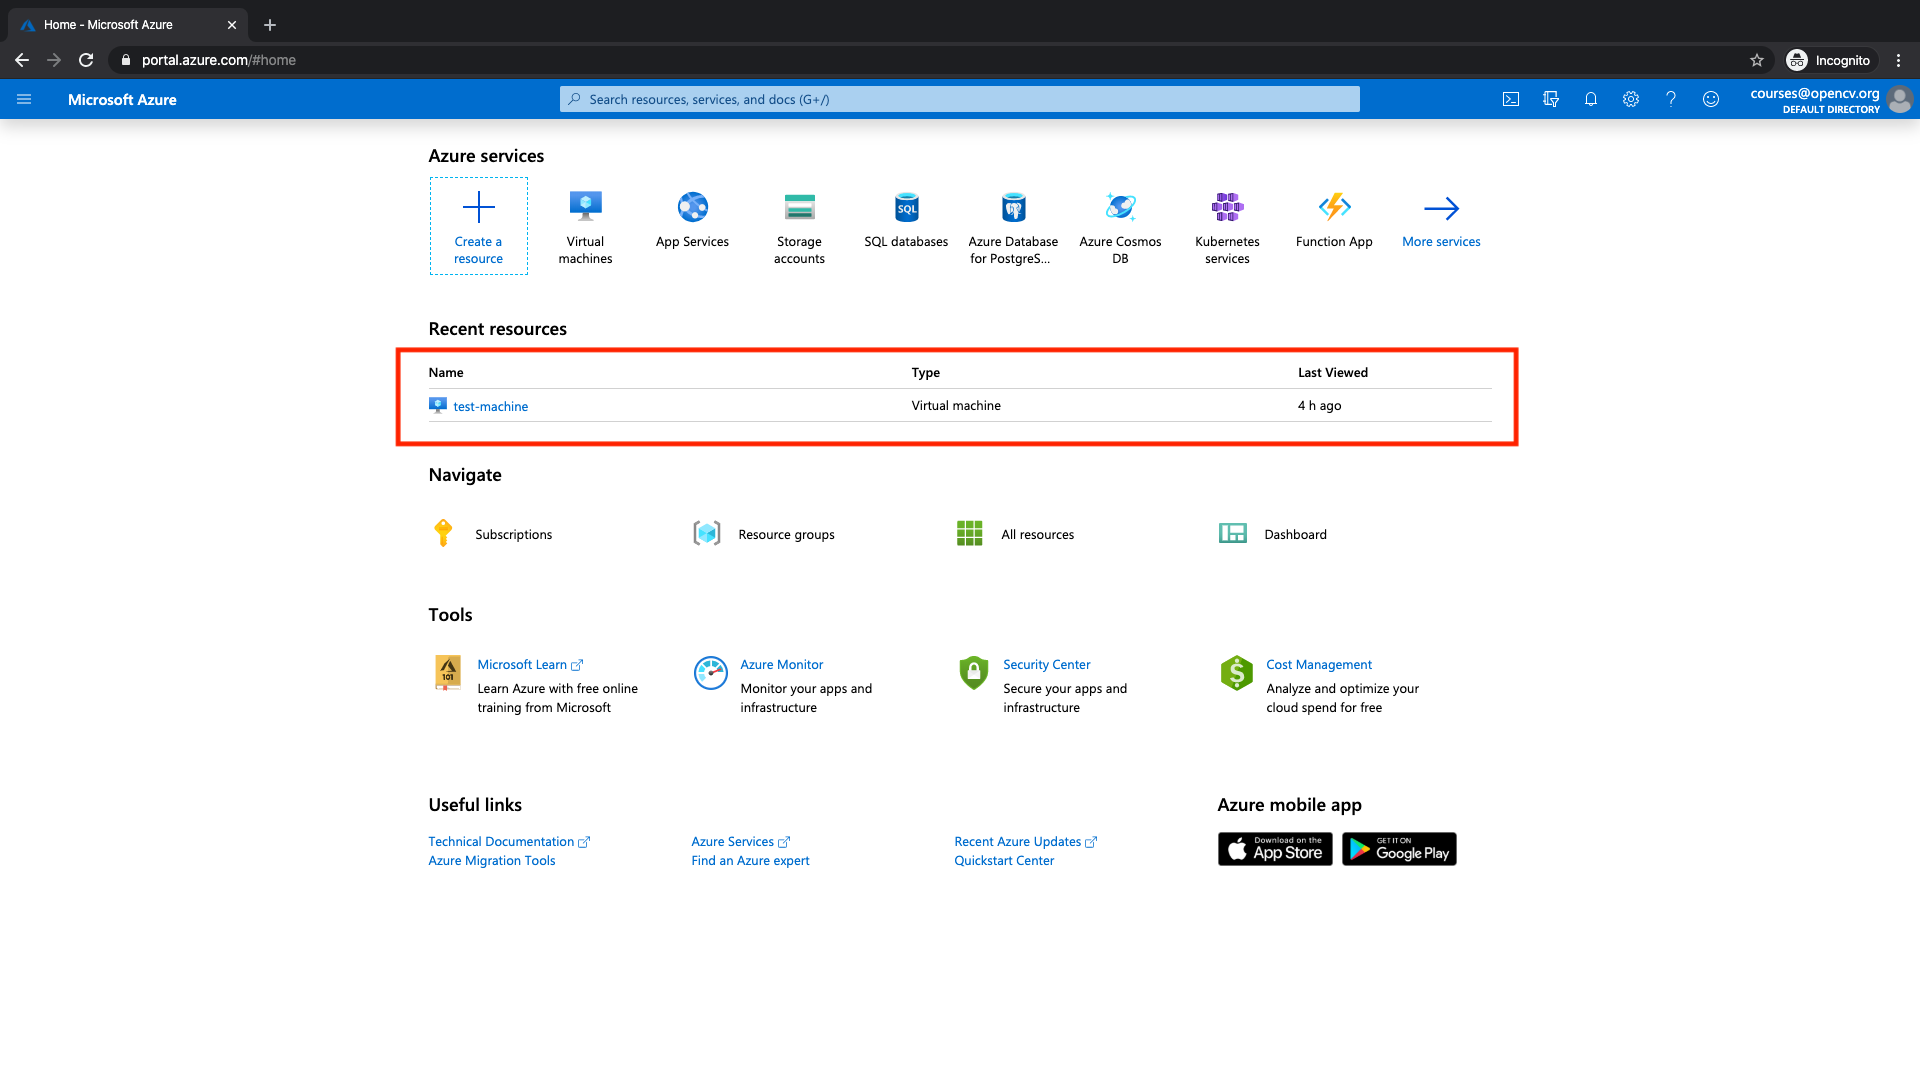
\includegraphics[scale=0.20]{figures/ssh1}
%\caption{\small \sl . \cite{Mallick m.fl. 2020} \label{fig:azure}}
\end{center}
\end{figure}

You will see the IP address of your instance as shown.

\begin{figure}[H]
\begin{center} 
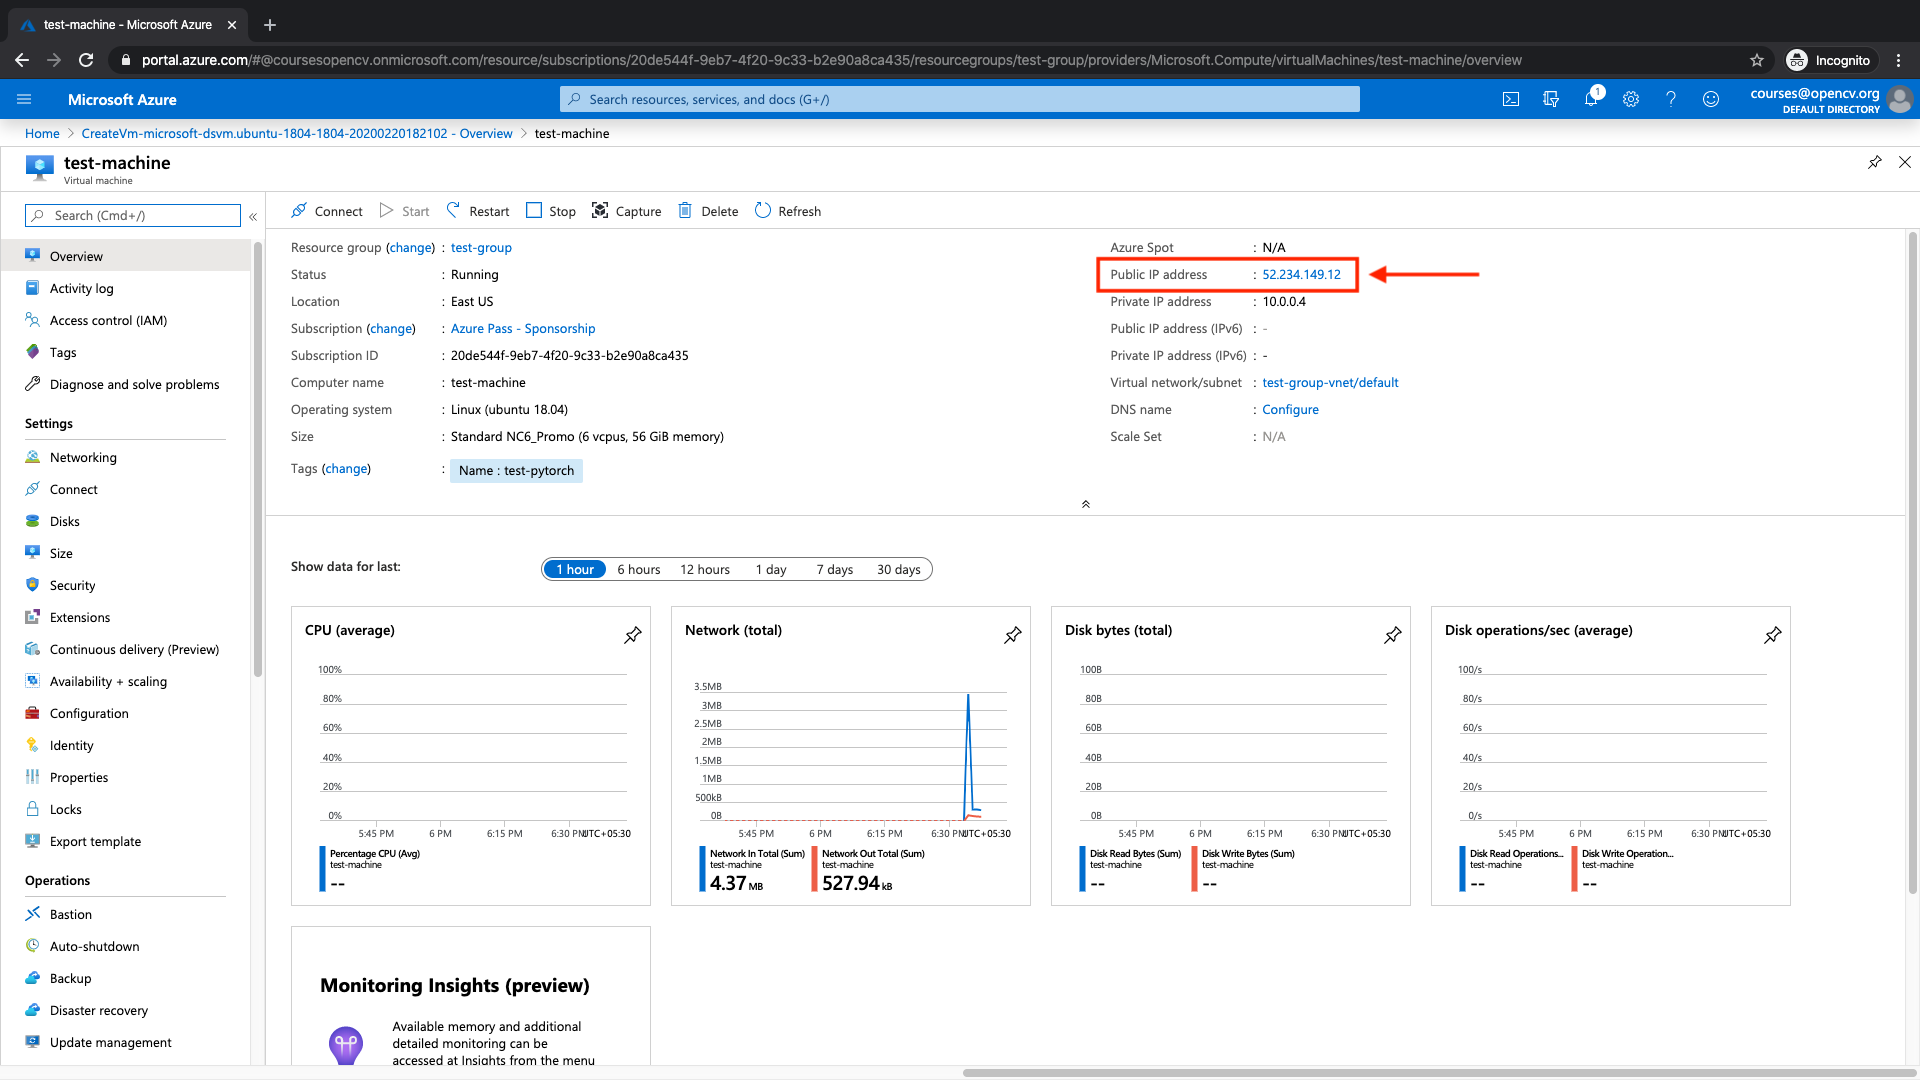
\includegraphics[scale=0.20]{figures/ssh2}
%\caption{\small \sl . \cite{Mallick m.fl. 2020} \label{fig:azure}}
\end{center}
\end{figure}

2. SSH into your instance
Start a terminal or command prompt and execute the following

ssh user-name@ip-address

Here, you have to replace user-name and ip-address with your username and IP address.

\begin{figure}[H]
\begin{center} 
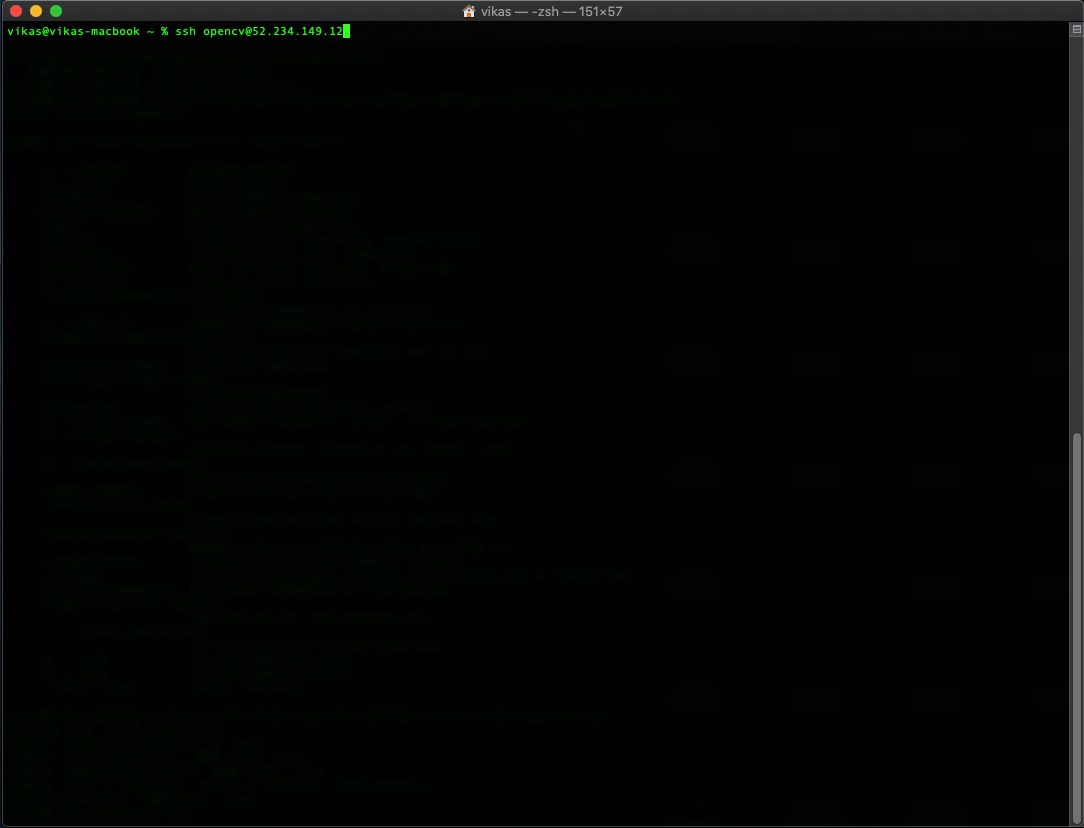
\includegraphics[scale=0.30]{figures/ssh3}
%\caption{\small \sl . \cite{Mallick m.fl. 2020} \label{fig:azure}}
\end{center}
\end{figure}

Since you are connecting to the instance for the first time, your system will ask you to add its fingerprint to your authorized\_keys file. 

\begin{figure}[H]
\begin{center} 
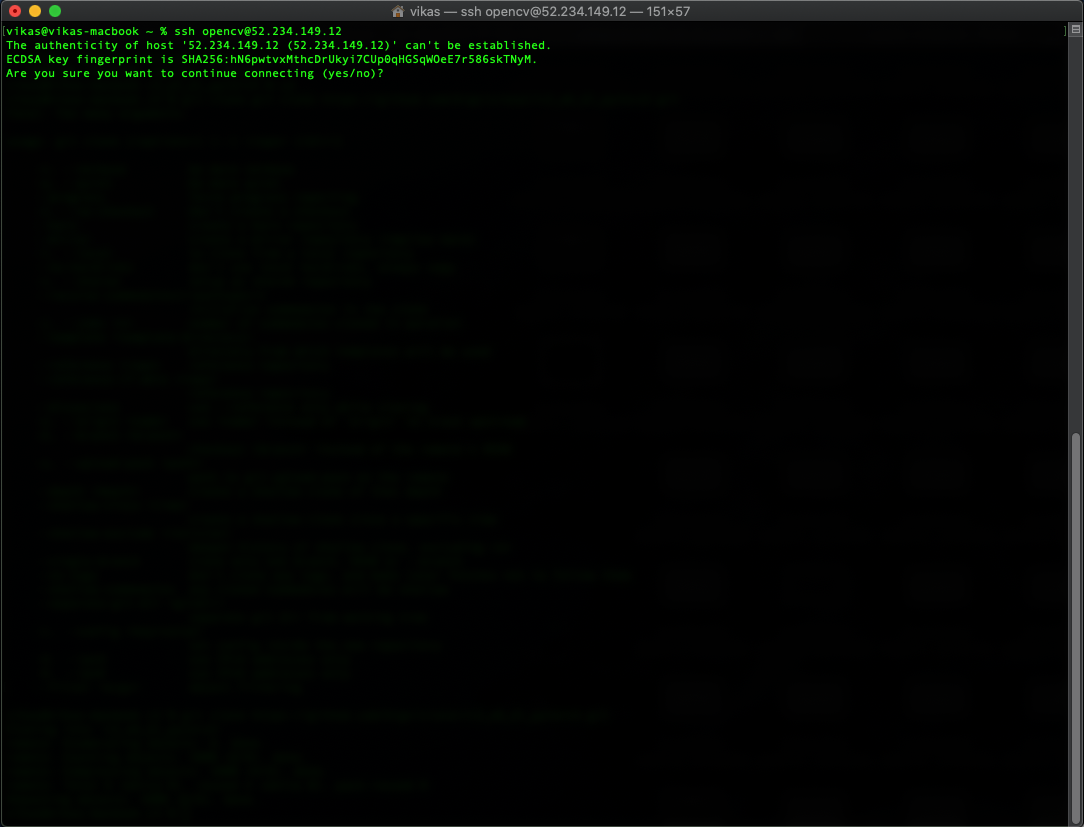
\includegraphics[scale=0.30]{figures/ssh4}
%\caption{\small \sl . \cite{Mallick m.fl. 2020} \label{fig:azure}}
\end{center}
\end{figure}

Accept it by typing yes and press Enter

\begin{figure}[H]
\begin{center} 
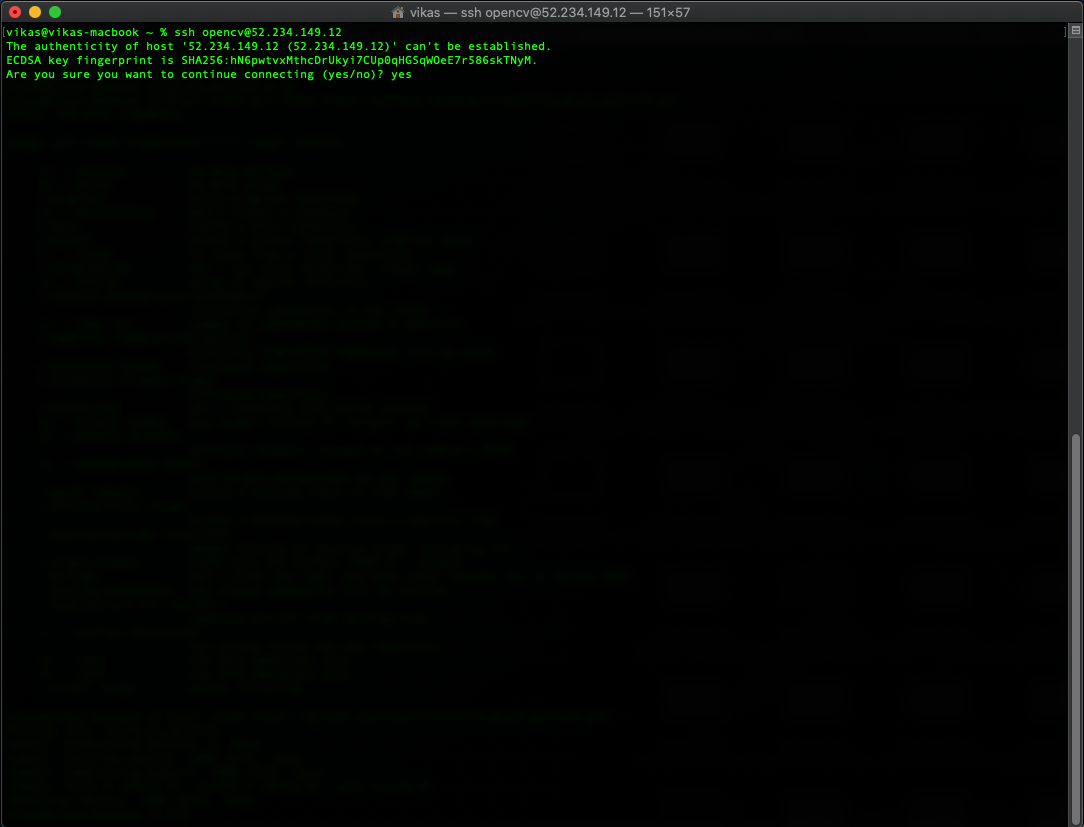
\includegraphics[scale=0.30]{figures/ssh5}
%\caption{\small \sl . \cite{Mallick m.fl. 2020} \label{fig:azure}}
\end{center}
\end{figure}

It will ask for the password. Type in the password you set while creating the instance.

\begin{figure}[H]
\begin{center} 
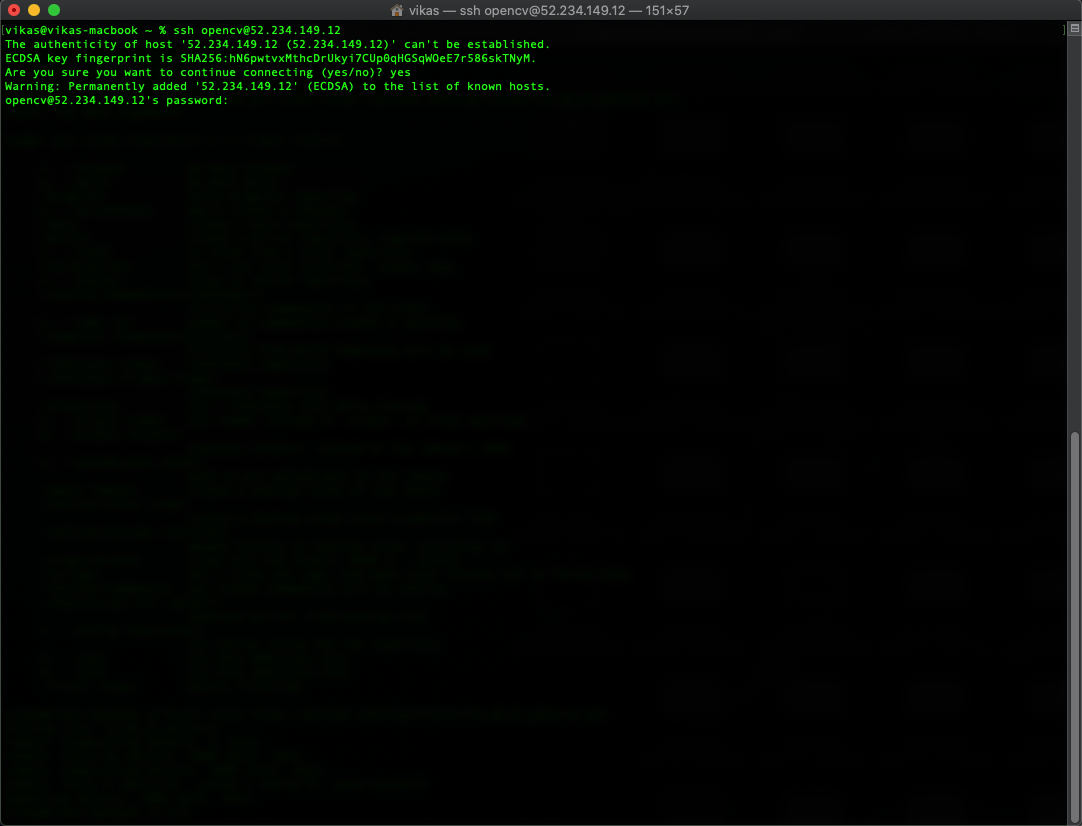
\includegraphics[scale=0.30]{figures/ssh6}
%\caption{\small \sl . \cite{Mallick m.fl. 2020} \label{fig:azure}}
\end{center}
\end{figure}

3. Explore
Once you login, you get a welcome message as shown below. You can see that it tells you that many conda environments are already installed and also how to use them.

\begin{figure}[H]
\begin{center} 
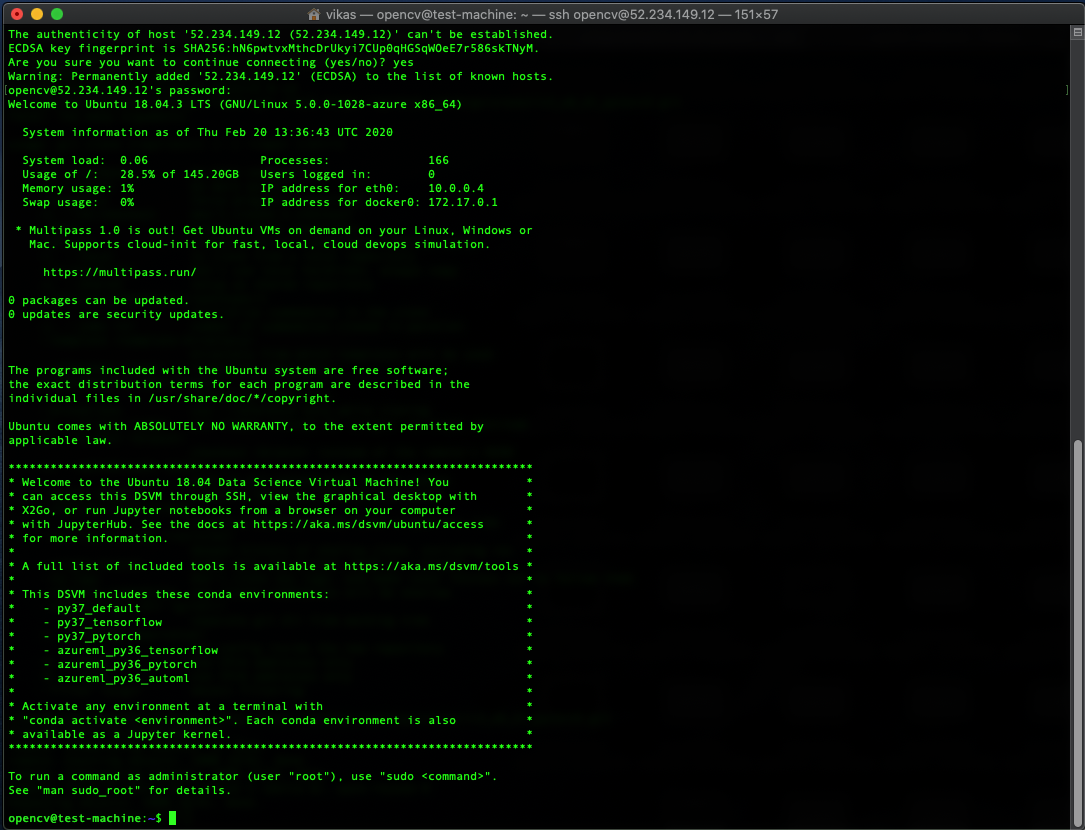
\includegraphics[scale=0.30]{figures/ssh7}
%\caption{\small \sl . \cite{Mallick m.fl. 2020} \label{fig:azure}}
\end{center}
\end{figure}

4. Check PyTorch
Let us open an ipython terminal and see if PyTorch is really installed?

\begin{figure}[H]
\begin{center} 
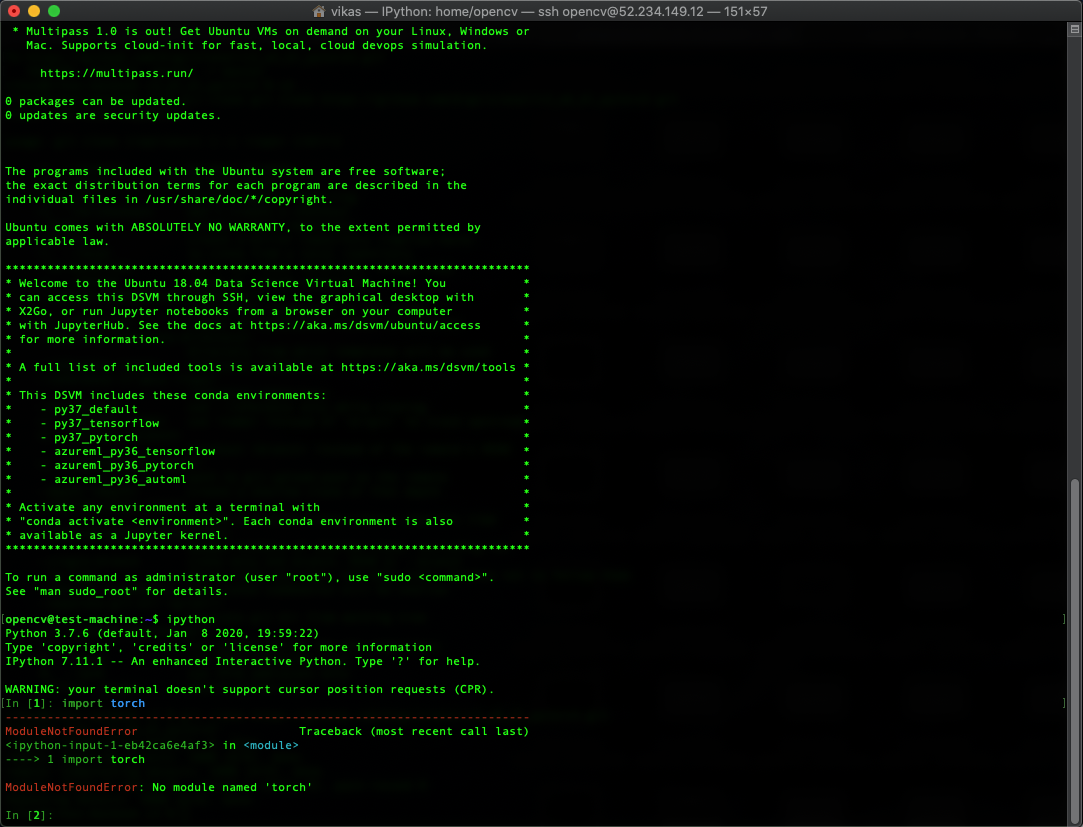
\includegraphics[scale=0.30]{figures/ssh8}
%\caption{\small \sl . \cite{Mallick m.fl. 2020} \label{fig:azure}}
\end{center}
\end{figure}

The error says Torch is not installed. This is because every library is installed in their respective conda environments as shown below.

\begin{figure}[H]
\begin{center} 
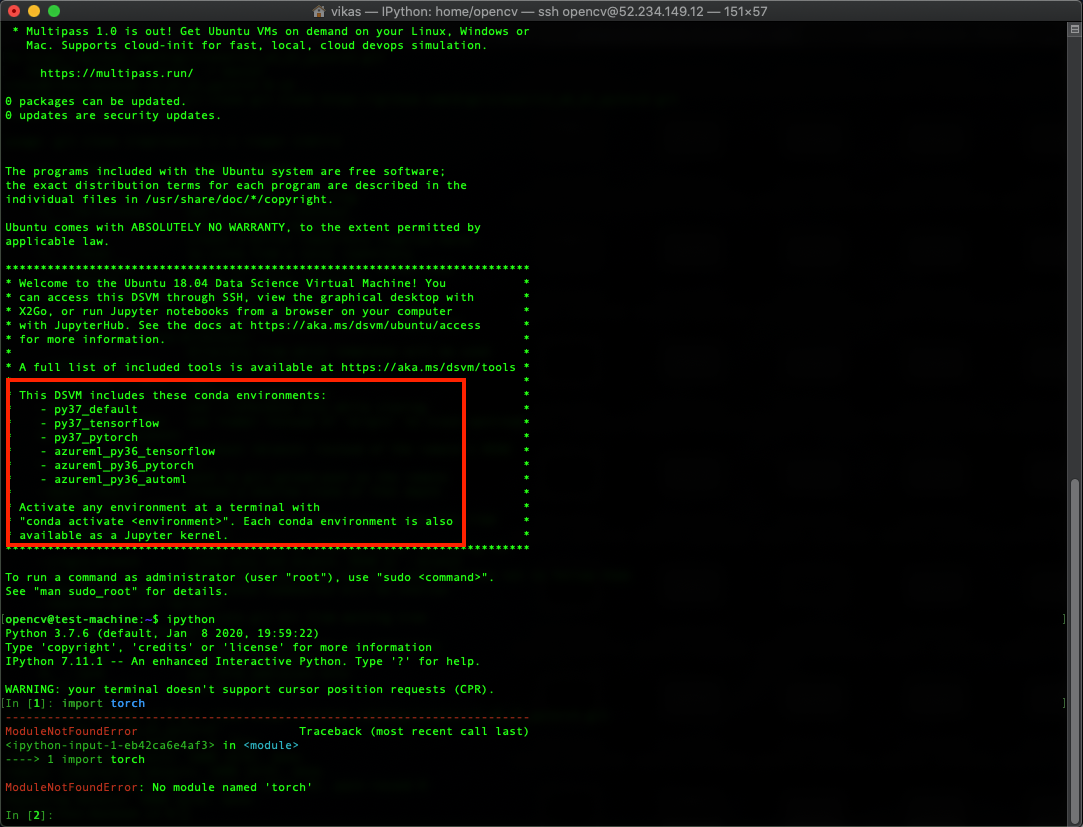
\includegraphics[scale=0.30]{figures/ssh9}
%\caption{\small \sl . \cite{Mallick m.fl. 2020} \label{fig:azure}}
\end{center}
\end{figure}

Let us activate a py37\_pytorch environment and check.

\begin{figure}[H]
\begin{center} 
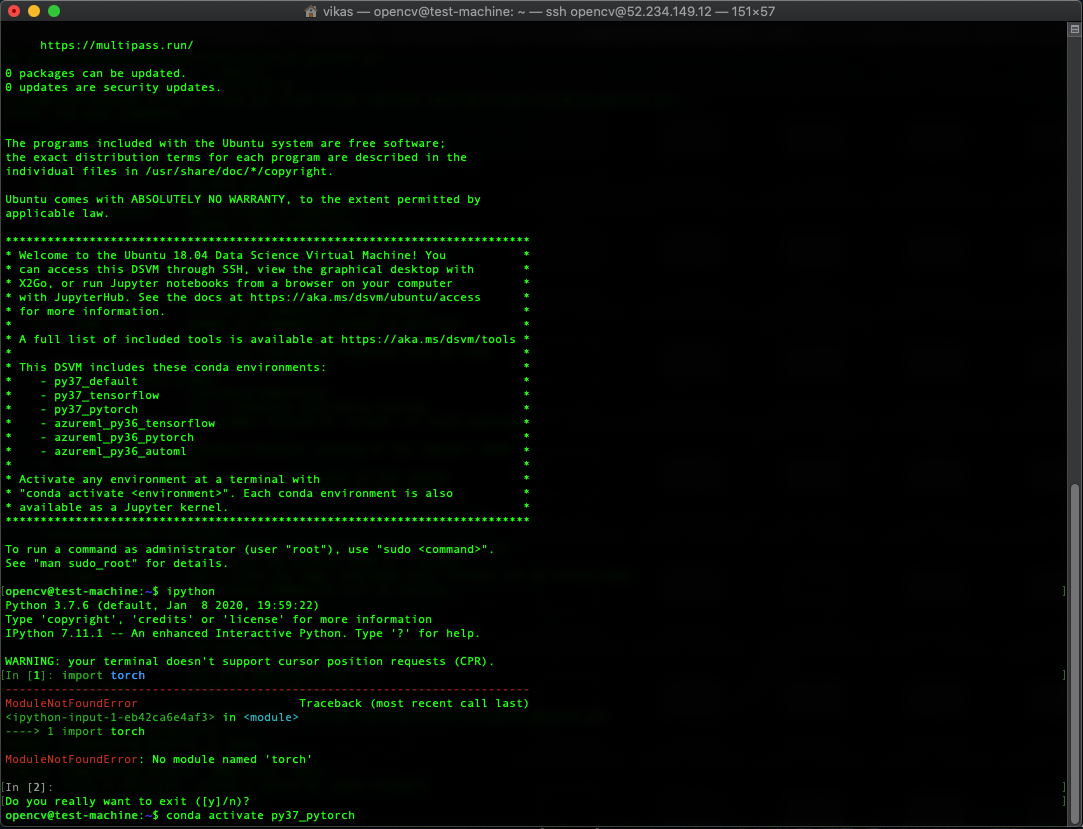
\includegraphics[scale=0.30]{figures/ssh10}
%\caption{\small \sl . \cite{Mallick m.fl. 2020} \label{fig:azure}}
\end{center}
\end{figure}

\begin{figure}[H]
\begin{center} 
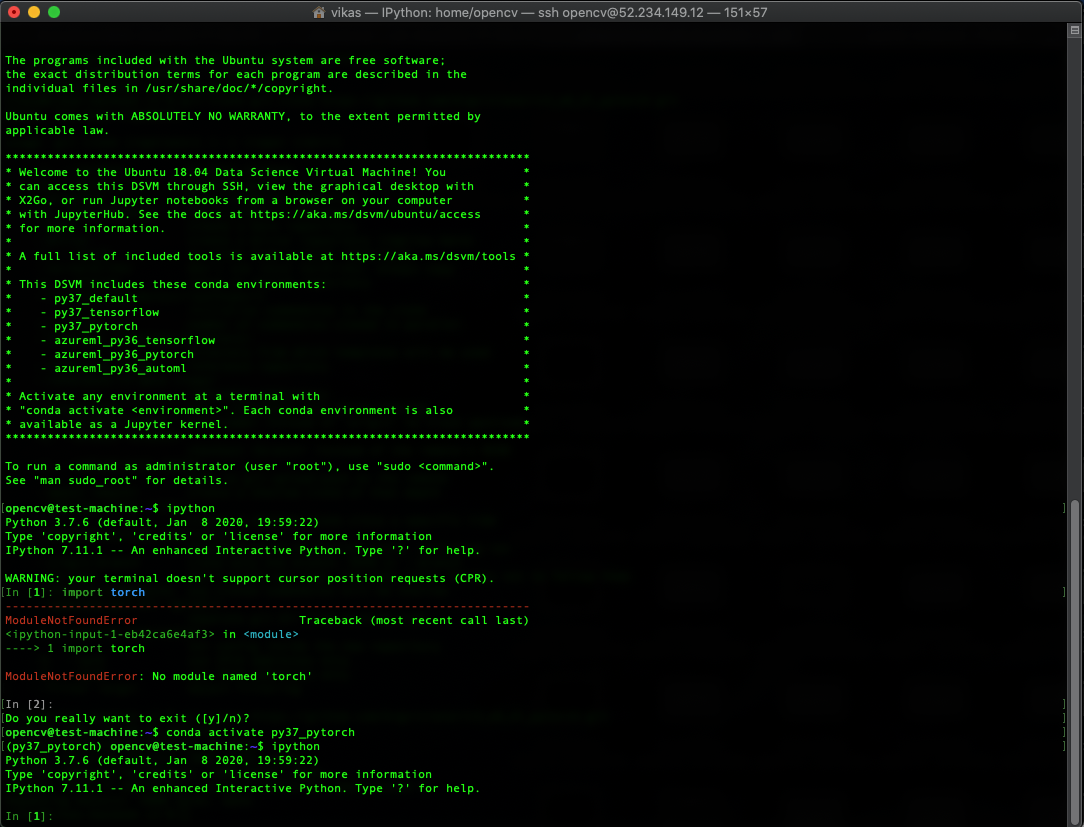
\includegraphics[scale=0.30]{figures/ssh11}
%\caption{\small \sl . \cite{Mallick m.fl. 2020} \label{fig:azure}}
\end{center}
\end{figure}

\begin{figure}[H]
\begin{center} 
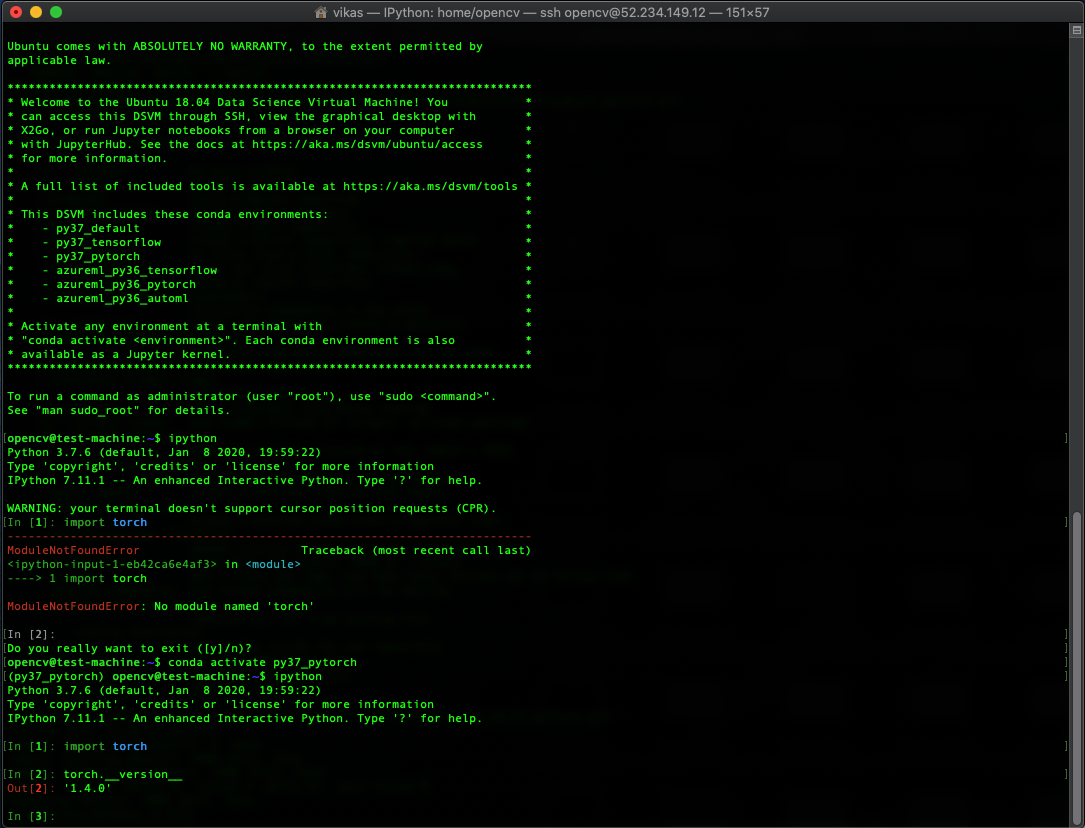
\includegraphics[scale=0.30]{figures/ssh12}
%\caption{\small \sl . \cite{Mallick m.fl. 2020} \label{fig:azure}}
\end{center}
\end{figure}

So, we have the latest version of PyTorch installed here.

Once you are done, exit the system

\begin{figure}[H]
\begin{center} 
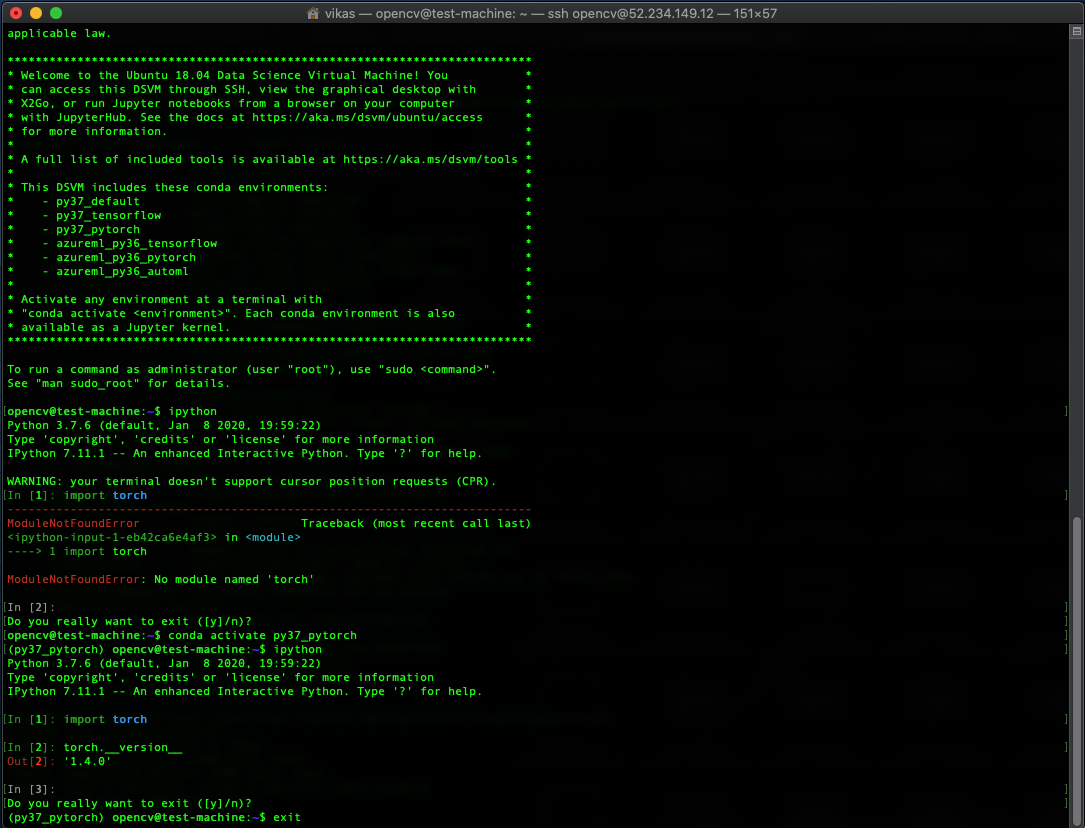
\includegraphics[scale=0.30]{figures/ssh13}
%\caption{\small \sl . \cite{Mallick m.fl. 2020} \label{fig:azure}}
\end{center}
\end{figure}

Note that exiting the system does not mean that the system is shut down. You need to shut it down manually from the Portal Dashboard.